\documentclass{article}


%%%
%PLOTS mapas y conglomerados
%Bibliografía
%%%
\usepackage[utf8]{inputenc}
\usepackage{longtable}
\usepackage{authblk}
\usepackage{adjustbox}
\usepackage{natbib}

\title{LOS INDICES DE COLOMBIA}
\author[1]{\normalsize Mario Andrés Cifuentes}
\affil[1,2]{\small  Departamento Ingeniería Industrial,Universidad de los Andes\\
\texttt{{ma.cifuentes10}@uniandes.edu.co}}

\date{29 de Junio de 2018}

\usepackage{Sweave}
\begin{document}
\Sconcordance{concordance:ProyectoFinal.tex:ProyectoFinal.Rnw:%
1 20 1 1 0 19 1 1 5 1 4 14 0 1 3 1 8 1 2 6 1 1 14 1 3 8 1 1 5 12 0 1 2 %
2 1 1 8 13 0 1 2 5 1 2 2 8 1 1 5 1 4 31 0 1 2 4 1 1 21 1 1 1 18 3 1 1 %
14 1 2 9 1}


\maketitle


\begin{abstract}
Este es el proyecto de aplicación de los contenidos vistos durante el curso de herramientas computacionales para investigación, en la Universidad de los Andes.
\end{abstract}

\section*{Introducción}

Aqui les presento mi investigacion sobre diversos indices sociales en el mundo. Los indices los conseguí de wikipedia, espero que les gusten mucho. Aqui les presento mi investigacion sobre diversos indices sociales en el mundo. Los indices los conseguí de wikipedia, espero que les gusten mucho.Aqui les presento mi investigacion sobre diversos indices sociales en el mundo. Los indices los conseguí de wikipedia, espero que les gusten mucho.Aqui les presento mi investigacion sobre diversos indices sociales en el mundo. Los indices los conseguí de wikipedia, espero que les gusten mucho.
Aqui les presento mi investigacion sobre diversos indices sociales en el mundo. Los indices los conseguí de wikipedia, espero que les gusten mucho.Aqui les presento mi investigacion sobre diversos indices sociales en el mundo. Los indices los conseguí de wikipedia, espero que les gusten mucho.Aqui les presento mi investigacion sobre diversos indices sociales en el mundo. Los indices los conseguí de wikipedia, espero que les gusten mucho.

\clearpage

\section{Exploración Univariada}\label{univariada}

En esta sección exploro cada índice. En esta sección exploro cada índice. En esta sección exploro cada índice. En esta sección exploro cada índice. En esta sección exploro cada índice. En esta sección exploro cada índice. En esta sección exploro cada índice. En esta sección exploro cada índice. En esta sección exploro cada índice.


% Table created by stargazer v.5.2.2 by Marek Hlavac, Harvard University. E-mail: hlavac at fas.harvard.edu
% Date and time: Fri, Jun 29, 2018 - 9:50:32 PM
\begin{table}[!htbp] \centering 
  \caption{Medias estadísticas} 
  \label{stats} 
\begin{tabular}{@{\extracolsep{5pt}}lcccc} 
\\[-1.8ex]\hline 
\hline \\[-1.8ex] 
Statistic & \multicolumn{1}{c}{N} & \multicolumn{1}{c}{Min} & \multicolumn{1}{c}{Median} & \multicolumn{1}{c}{Max} \\ 
\hline \\[-1.8ex] 
IDH & 32 & 0.691 & 0.804 & 0.879 \\ 
Población.Cabecera & 32 & 13,090 & 717,197 & 10,070,801 \\ 
Población.Resto & 32 & 21,926 & 268,111.5 & 1,428,858 \\ 
\hline \\[-1.8ex] 
\end{tabular} 
\end{table} 
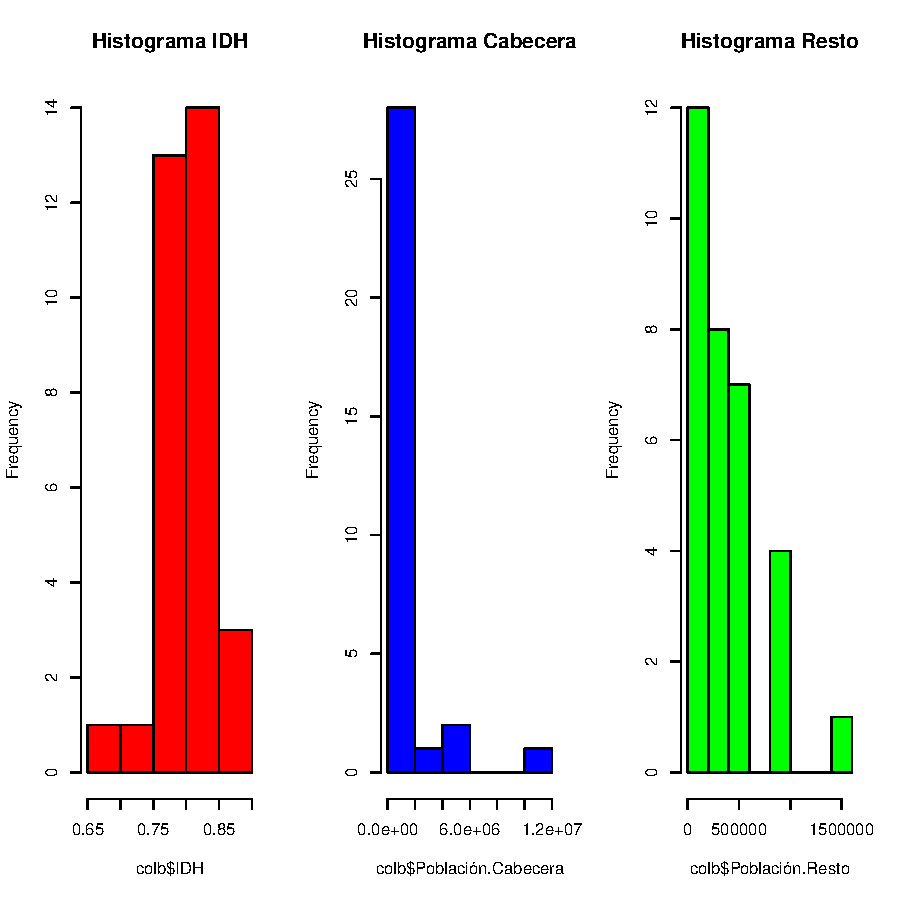
\includegraphics{ProyectoFinal-Histogramas}

Hay que tener en cuenta que los datos acerca de las poblaciones pueden llegar a estar sesgados, por lo cual se pueden corrgir este error mediante la normalización de los datos que se presenta a continuación.


\begin{figure}[h]
\centering
\begin{adjustbox}{width=7cm,height=7cm,clip,trim=1.5cm 0.5cm 0cm 1.5cm}
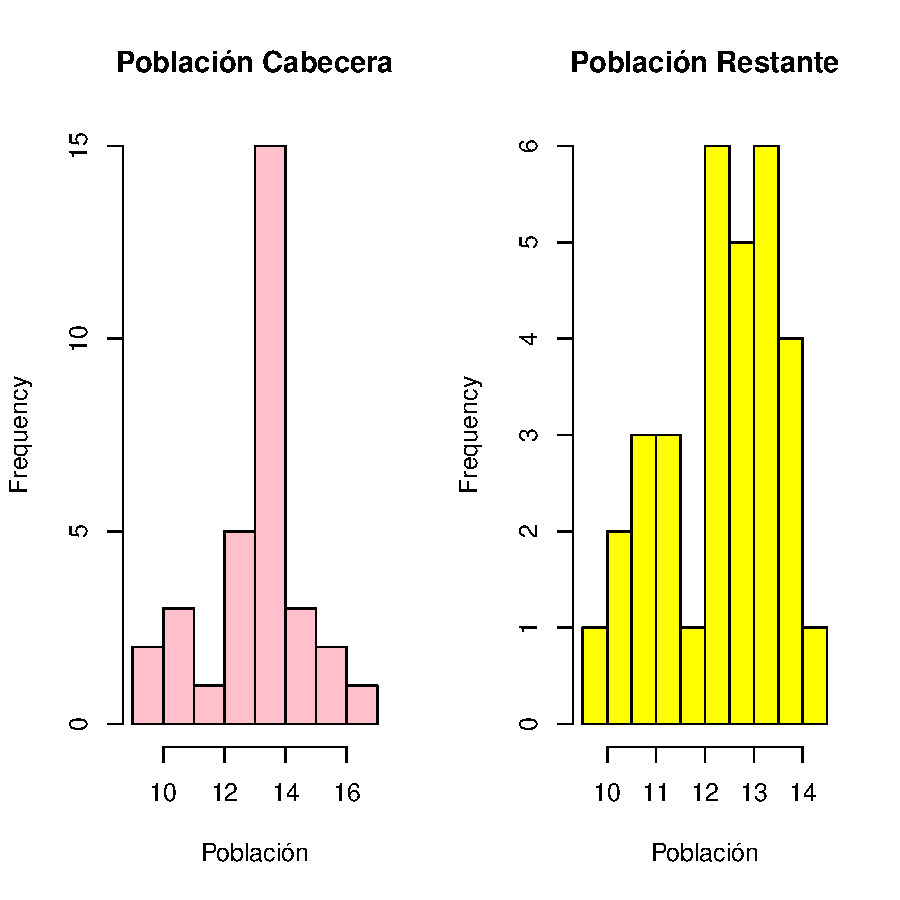
\includegraphics{ProyectoFinal-Normalizados}
\end{adjustbox}
\caption{Histogramas Población Normalizados }
\label{histplotsNorm}
\end{figure}

\section{Exploración Bivariada}\label{bivariada}

Ahora se analizará el impacto que tienen otros indices, mediante el estudio de las relaciones bivariadas.

% Table created by stargazer v.5.2.2 by Marek Hlavac, Harvard University. E-mail: hlavac at fas.harvard.edu
% Date and time: Fri, Jun 29, 2018 - 9:50:47 PM
\begin{table}[!htbp] \centering 
  \caption{Correlación de Democracia con las demás variables} 
  \label{corrDem} 
\begin{tabular}{@{\extracolsep{5pt}} cc} 
\\[-1.8ex]\hline 
\hline \\[-1.8ex] 
cabeLog & restoLog \\ 
\hline \\[-1.8ex] 
$0.487$ & $0.177$ \\ 
\hline \\[-1.8ex] 
\end{tabular} 
\end{table} 
Ahora se estudiara la correlación entre variables independientes:

% Table created by stargazer v.5.2.2 by Marek Hlavac, Harvard University. E-mail: hlavac at fas.harvard.edu
% Date and time: Fri, Jun 29, 2018 - 9:50:47 PM
\begin{table}[!htbp] \centering 
  \caption{Correlación de variables independientes} 
  \label{corrTableX} 
\begin{tabular}{@{\extracolsep{5pt}} ccc} 
\\[-1.8ex]\hline 
\hline \\[-1.8ex] 
 & cabeLog & restoLog \\ 
\hline \\[-1.8ex] 
cabeLog & 1 &  \\ 
restoLog & 0.8 & 1 \\ 
\hline \\[-1.8ex] 
\end{tabular} 
\end{table} 
A la tabla anterior se le relaciona la siguiente gráfica:

\begin{figure}[h]
\centering
\begin{adjustbox}{}
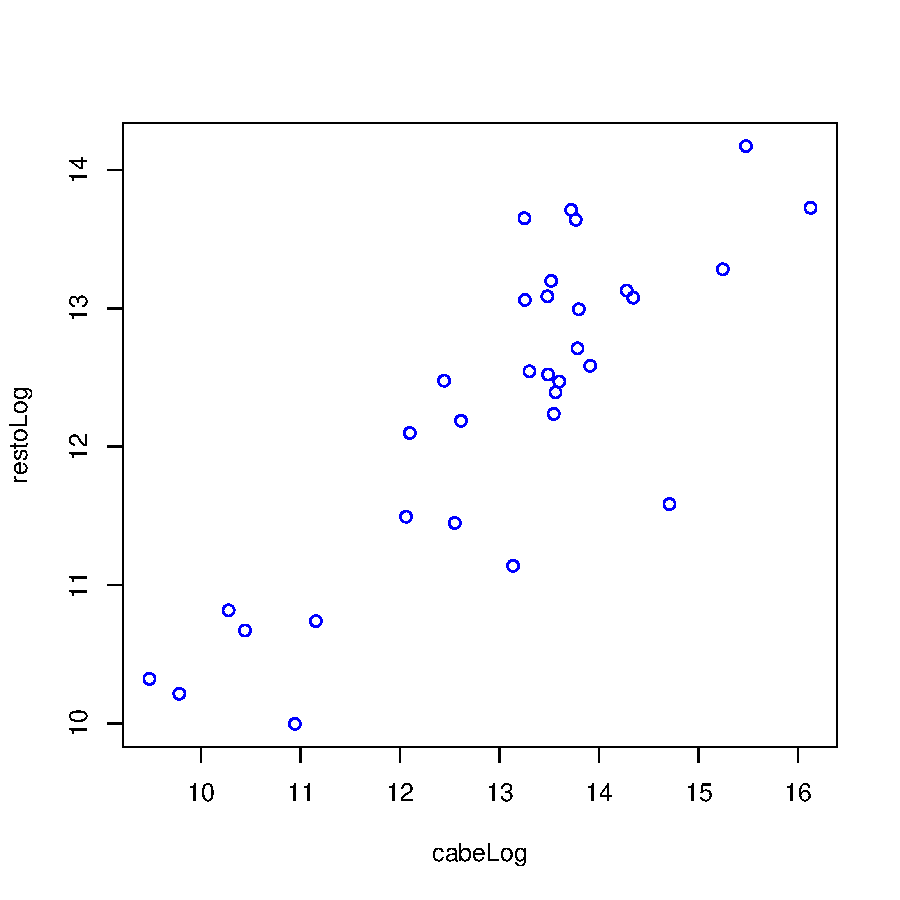
\includegraphics{ProyectoFinal-corrPlotX}
\end{adjustbox}
\caption{Correlación entre variables significativas}
\label{corrPlotX}
\end{figure}

\section{Modelos de Regresión}\label{modelos}

Ahora se analizarán los distintos modelos propuestos para el caso de estudio.


% Table created by stargazer v.5.2.2 by Marek Hlavac, Harvard University. E-mail: hlavac at fas.harvard.edu
% Date and time: Fri, Jun 29, 2018 - 9:50:47 PM
\begin{table}[!htbp] \centering 
  \caption{Modelos de Regresión} 
  \label{regresiones} 
\begin{tabular}{@{\extracolsep{5pt}}lcc} 
\\[-1.8ex]\hline 
\hline \\[-1.8ex] 
 & \multicolumn{2}{c}{\textit{Dependent variable:}} \\ 
\cline{2-3} 
\\[-1.8ex] & \multicolumn{2}{c}{IDH} \\ 
\\[-1.8ex] & (1) & (2)\\ 
\hline \\[-1.8ex] 
 cabeLog & 0.013$^{***}$ & 0.031$^{***}$ \\ 
  & (0.004) & (0.007) \\ 
  & & \\ 
 restoLog &  & $-$0.030$^{***}$ \\ 
  &  & (0.010) \\ 
  & & \\ 
 Constant & 0.634$^{***}$ & 0.766$^{***}$ \\ 
  & (0.055) & (0.065) \\ 
  & & \\ 
\hline \\[-1.8ex] 
Observations & 32 & 32 \\ 
R$^{2}$ & 0.238 & 0.425 \\ 
Adjusted R$^{2}$ & 0.212 & 0.385 \\ 
Residual Std. Error & 0.037 (df = 30) & 0.033 (df = 29) \\ 
F Statistic & 9.347$^{***}$ (df = 1; 30) & 10.706$^{***}$ (df = 2; 29) \\ 
\hline 
\hline \\[-1.8ex] 
\textit{Note:}  & \multicolumn{2}{r}{$^{*}$p$<$0.1; $^{**}$p$<$0.05; $^{***}$p$<$0.01} \\ 
\end{tabular} 
\end{table} 
\section{Exploración Espacial}\label{exploracion}

Se calcuaran los conglomerados por regiones usando la información disponible de las variables significativas para el problema. Se utilizará la técnica de k-means propuesta por \cite{macqueen_methods_nodate}.




\begin{figure}[h]
\centering
\begin{adjustbox}{width=12cm,height=12cm,clip,trim=0cm 0cm 0cm 0cm}
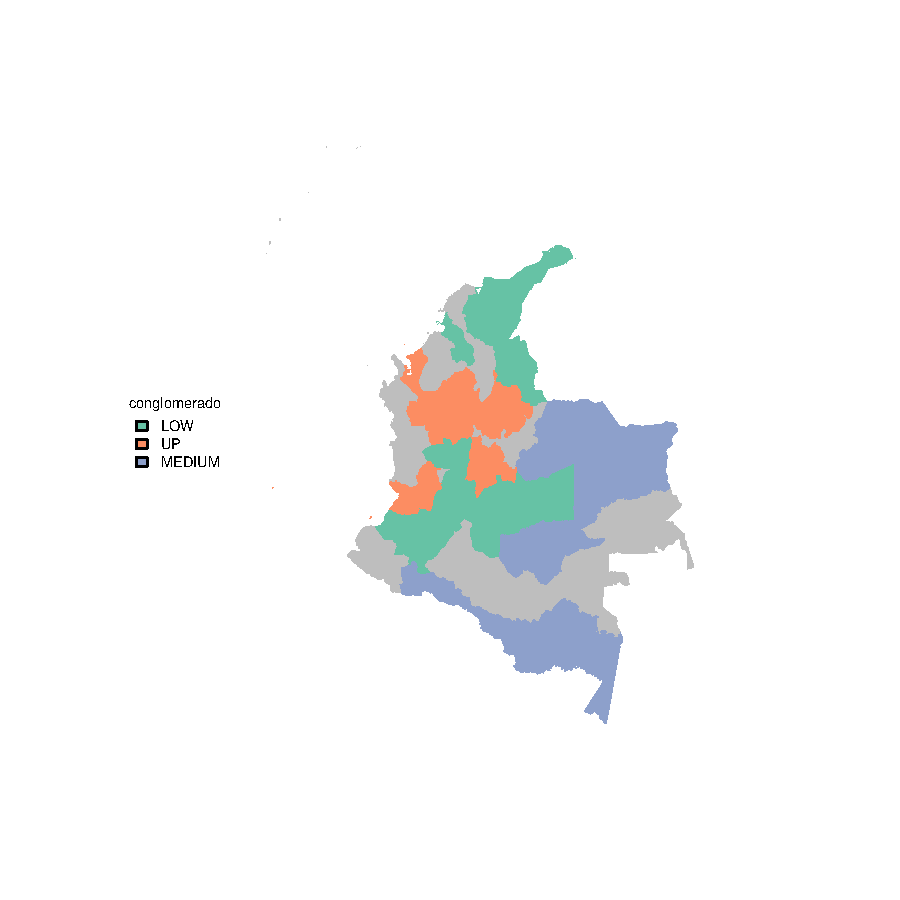
\includegraphics{ProyectoFinal-plotMap1}
\end{adjustbox}
\caption{Departamentos según sus indicadores}\label{clustmap}
\end{figure}


\bibliographystyle{abbrv}
%\renewcommand{\refname}{Bibliografía}
\bibliography{proyecto}

\end{document}
